\section{Introduction}

\begin{quote}
	\textit{Solomon,\\ I'm concerned about security; I think, when we email each other, we should use some sort of code.}
\end{quote}

Confidentiality is our goal.
We want to encrypt and decrypt a (plaintext) message $m$, using a key, to obtain a cyphertext $c$.
As per Kirkoff's principle, only the key is secret.

\begin{figure}
	\centering
	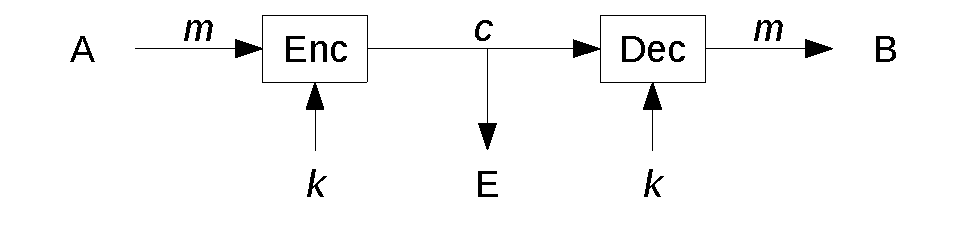
\includegraphics[width=0.8\linewidth]{drawings/symmetric-encryption.eps}
	\caption{Message exchange between $A$ and $B$ using symmetric encryption. $E$ is the eavesdropper.}
	\label{fig:symmetric-encryption}
\end{figure}

Our encryption schemes have the following syntax:
\begin{equation*}
	\GenericEncSchemeTuple.
\end{equation*}
$A$ and $B$, the actors of our communication exchange (\cref{fig:symmetric-encryption}), share $k$, the key, taken from some key space $\K$.
The elements of our encryption scheme play the following roles:
\begin{enumerate}
	\item $\GenericKeyGen$ outputs a random key from the key space $\K$, and we write this as $k \rand{\GenericKeyGen}$;
	\item $\GenericEnc : \K \times \M \to \C$ is the encryption function, mapping a key and a message to a cyphertext\footnote{In cryptography, ciphertext or cyphertext is the result of encryption performed on plaintext using an algorithm, called a cipher. Ciphertext is also known as encrypted or encoded information because it contains a form of the original plaintext that is unreadable by a human or computer without the proper cipher to decrypt it.};
	\item $\GenericDec : \K \times \C \to \M$ is the decryption function, mapping a key and a cyphertext to a message.
\end{enumerate}
We expect an encryption scheme to be at least correct:
\begin{equation*}
	\forall k \in \K, \forall m \in \M . \GenericDec(k, \GenericEnc(k, m)) = m.
\end{equation*}
An encryption scheme is defined by three algorithms $\GenericKeyGen$, $\GenericEnc$, and $\GenericDec$, as well as a specification of a message space $\M$ with $| \M | > 1$.\footnote{If $| M | = 1$ there is only one message and there is no point in communicating, let alone encrypting.}
\subsection{Perfect secrecy}

Shannon defined ``perfect secrecy'', \ie the fact that the cyphertext carries no information about the plaintext.
\begin{definition}[Perfect secrecy]\label{def:perfect-secrecy}
	Let $M$ be a \ac{RV} over $\M$, and $K$ be a uniform distribution over $\K$.

	$(\GenericEnc, \GenericDec)$ has perfect secrecy if
	\begin{equation*}
		\forall M, \forall m \in \M, c \in \C . \Pr{M = m} = \Pr{M = m | C = c}
	\end{equation*}
	where $C = \GenericEnc(k,m)$ is a third \ac{RV}.
\end{definition}

We have equivalent definitions for perfect secrecy.
\begin{theorem}\label{thm:perfect-secrecy:equivalent-definitions}
	The following definitions are equivalent:
	\begin{enumerate}
		\item \label{itm:thm:perfect-secrecy:original} \cref{def:perfect-secrecy}:
		\begin{equation*}
			\Pr{M = m} = \Pr{M = m | C = c}
		\end{equation*}
		\item \label{itm:thm:perfect-secrecy:independent} $M$ and $C$ are independent;
		\item \label{itm:thm:perfect-secrecy:invariant}
		$\forall m, m' \in \M, \forall c \in \C \quad \footnote{The encryption algorithm may be probabilistic, so that $\GenericEnc(m)$ might output a different ciphertext when run multiple times. To emphasize this, we write $c \leftarrow \GenericEnc(m)$ to denote the possibly probabilistic process by which message $m$ is encrypted using key $k$ to give ciphertext $c$.}:$
			\begin{equation*}
				\Pr{\GenericEnc(k,m) = c} = \Pr{\GenericEnc(k,m') = c}
			\end{equation*}
			where $k$ is a random key in $\K$ chosen with uniform probability. \qedhere
	\end{enumerate}
\end{theorem}

\begin{proof}[Proof of \cref{thm:perfect-secrecy:equivalent-definitions}]
	First, we show that \ref{itm:thm:perfect-secrecy:original} implies \ref{itm:thm:perfect-secrecy:independent}.
	\begin{align*}
		\Pr{M=m} & = \Pr{M = m | C = c} \\
		& = \frac{\Pr{M = m \land C = c}}{\Pr{C = c}} \tag{by Bayes}
		\\
		& \implies \\
		\Pr{M = m} \Pr{C = c}
		& =
		\Pr{M = m \land C = c}
	\end{align*}
	which is the definition of independence.

	Now we show that \ref{itm:thm:perfect-secrecy:independent} implies \ref{itm:thm:perfect-secrecy:invariant}.
	\begin{align*}
		\Pr{\GenericEnc(k, m) = c} 
		& =
		\Pr{\GenericEnc(k, M) = c | M = m} \tag{we fixed $m$}
		\\
		& = \Pr{C = c | M = m} \tag{definition of the \ac{RV} $C$}
		\\
		& = \Pr{C = c}. \tag{by \ref{itm:thm:perfect-secrecy:independent}}
	\end{align*}
	Since $m$ is arbitrary, we can do the same for $m'$, and obtain
	\begin{equation*}
		\Pr{\GenericEnc(k,m') = c} = \Pr{C = c}
	\end{equation*}
	which gives us \ref{itm:thm:perfect-secrecy:invariant}.

	Now we want to show that \ref{itm:thm:perfect-secrecy:invariant} implies \ref{itm:thm:perfect-secrecy:original}. Assume that the encryption scheme is perfectly secret and fix messages $m$, $m\prime$ $\in \M$ and a ciphertext $c \in \C$. Take any $c \in \C$. By \ref{itm:thm:perfect-secrecy:independent} we have:

	\begin{equation*}
		\Pr {C = c | M = m} = \Pr {C = c} = \Pr {C = c | M = m'}.
	\end{equation*}

	completing the proof of the first direction.
	Assume next that for every distribution over $\M$, every $m$, $m\prime \in \M$, and every $c \in \C$ it holds that $\Pr {C = c | M = m} = \Pr {C = c | M = m\prime}$. Fix some distribution over $\M$, and an arbitrary $m \in \M$ and $c \in \C$. Define $p \stackrel{\text{def}}{=}$ $\Pr {C = c | M = m}$. Since $\Pr {C = c | M = m} = \Pr {C = c | M = m'} = p$ for all $m$, we have:

	\begin{align*}
		\Pr{C = c}
		& =
		\sum_{m' \in \M} \Pr{C = c \land M = m'}
		\\
		& = 
		\sum_{m' \in \M} \Pr{C = c | M = m'} \Pr{M = m'}
		\tag{by Bayes}
		\\
		& =
		\sum_{m' \in \M} \Pr{\GenericEnc(k,M) = c | M = m'} \Pr{M = m'}
		\\
		& =
		\sum_{m' \in \M} \Pr{\GenericEnc(k,m') = c} \Pr{M = m'}
		\\
		& =
		\Pr{\GenericEnc(k, m) = c} \underbrace{\sum_{m' \in \M} \Pr{M = m'}}_{1}
		\tag{$\GenericEnc$ is indepenendent of $M$, so we take it out}
		\\
		& =
		\Pr{\GenericEnc(k,M) = c | M = m} =
		\Pr{C = c | M = m}.
	\end{align*}
	We are left to show that $\Pr{M = m} = \Pr{M = m | C = c}$, but this is easy with Bayes.
\end{proof}

\subsection{\acl{OTP}}

Now we'll see a perfect encryption scheme, the \ac{OTP}.

\begin{construction}[\acl{OTP}]
	The message space, the cyphertext space, and the key space are all the same, \ie $\M = \K = \C = \{0,1\}^{l}$, with $l \in \Naturals$.

	Encryption and decryption use the xor operation:
	\begin{itemize}
		\item $\OTPEnc(k,m) = k \xor m = c$;
		\item $\OTPDec(k,c) = c \xor k = (k \xor m) \xor k = m$.
	\end{itemize}
\end{construction}
Seeing that this is correct is immediate.

This can actually be done in any finite abelian group $(\Group, +)$, where you just do $k + m$ to encode and $c - k$ to decode.

\begin{theorem} \label{thm:otp:perfect-secrecy}
	\ac{OTP} is perfectly secure.
\end{theorem}

\begin{proof}[Proof of \cref{thm:otp:perfect-secrecy}]
	Fix $m \in \M, c \in \C$, and choose a random key.
	\begin{equation*}
		\Pr{\OTPEnc(k,m) = c} = \Pr{k = c - m} = \frac{1}{\abs{\Group}}.
	\end{equation*}
	This is true for any $m$, so we are done.
\end{proof}

\ac{OTP} has two problems:
\begin{enumerate}
	\item the key is long (as long as the message);
	\item we can't reuse the key:
	\begin{equation*}
		\begin{array}{c}
			c = k + m \\
			c' = k + m'
		\end{array}
		\implies
		c - c' = m - m'
		\implies
		m' = m - (c - c').
	\end{equation*}
\end{enumerate}

\begin{theorem}[Shannon, 1949] \label{thm:shannon:1949}
	In any perfectly secure encryption scheme the size of the key space is at least as large as the size of the message space, \ie $\abs{\K} \ge \abs{\M}$.
\end{theorem}

\begin{proof}[Proof of \cref{thm:shannon:1949}]
	Assume, for the sake of contradiction, that $\abs{\K} < \abs{\M}$.
	Fix $M$ to be the uniform distribution over $\M$, which we can do as perfect secrecy works for any distribution.
	Take a cyphertext $c \in \C$ such that $\Pr{C = c} > 0$, \ie $\exists m, k$ such that $\OTPEnc(k,m) = c$.

	Consider $\M' = \{ \OTPDec(k,c) : k \in \K \}$, the set of all messages decrypted from $c$ using any key.
	Clearly, $\abs{\M'} \le \abs{\K} < \abs{\M}$, so $\exists m' \in \M$ such that $m' \not\in \M'$.
	This means that
	\begin{equation*}
		\Pr{M = m'} = \frac{1}{\abs{\M}} \neq \Pr{M = m' | C = c} = 0
	\end{equation*}
	in contradiction with perfect secrecy.
\end{proof}

In the rest of the course we will forget about perfect secrecy, and strive for computational security, \ie bound the computational power of the adversary.

\subsection{Authentication}

The aim of authentication is to avoid tampering of $E$ with the messages exchanged between $A$ and $B$ (\cref{fig:symmetric-authentication}).

\begin{figure}
	\centering
	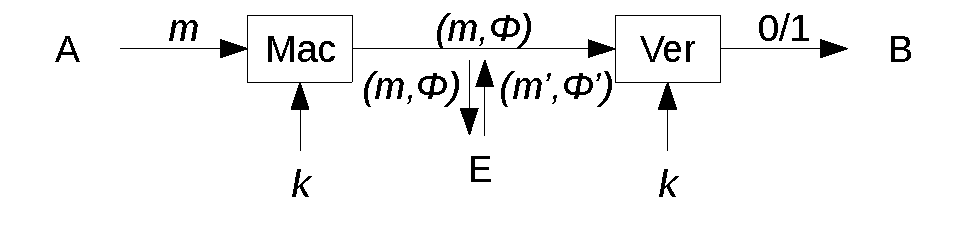
\includegraphics[width=0.8\linewidth]{drawings/symmetric-authentication.eps}
	\caption{Message exchange between $A$ and $B$ using symmetric authentication. $E$ is the eavesdropper.}
	\label{fig:symmetric-authentication}
\end{figure}

A \ac{MAC} is defined as a tuple $\GenericMACSchemeTuple$, where:
\begin{itemize}
	\item $\GenericKeyGen$, as usual, outputs a random key from some key space $\K$;
	\item $\GenericMac : \K \times \M \to \GenericAuthSpace$ maps a key and a message to an authenticator in some authenticator space $\GenericAuthSpace$;
	\item $\GenericVrfy : \K \times \M \times \GenericAuthSpace \to \Bool$ verifies the authenticator.
\end{itemize}
As usual, we expect a \ac{MAC} to be correct, \ie
\begin{equation*}
	\forall m \in \M, \forall k \in \K . \GenericVrfy(k, m, \GenericMac(k, m)) = 1.
\end{equation*}

If the $\GenericMac$ function is deterministic, then it must be that $\GenericVrfy(k, m, \phi) = 1$ if and only if $\GenericMac(k, m) = \phi$.

Security for \acp{MAC} is that \emph{forgery} must be hard: you can't come up with an authenticator for a message if you don't know the key.

\begin{definition}[Information theoretic \acs{MAC}]
	$(\GenericMac, \GenericVrfy)$ has $\epsilon$-statistical security if for all (possibly unbounded) adversary $\Adv$, for all $m \in \M$,
	\begin{equation*}
		\Pr{
			\GenericVrfy(k, m', \phi') = 1 \land m' \neq m :
			\begin{array}{l}
				k \rand{\KeyGen}; \; \\
				\phi = \GenericMac(k,m); \; \\
				(m', \phi') \from \Adv(m,\phi)
			\end{array}
		} \le \epsilon
	\end{equation*}
	\ie the adversary forges a $(m',\phi')$ that verifies with key $k$ with low probability, even if it knows a valid pair $(m, \phi)$.
\end{definition}

As an exercise, prove that the above is impossible if $\epsilon = 0$.

Information theoretic security is also called unconditional security.
Later we'll see \emph{conditional} security, based on computational assumptions.

\begin{definition}[Pairwise independence]
	Given a family $\H = \{ h_k : \M \to \GenericAuthSpace \}_{k \in \K}$ of functions, we say that $\H$ is pairwise independent if for all distinct $m, m'$ we have that $(h_k(m), h_k(m')) \in \GenericAuthSpace^2$ is uniform over the choice of $k \rand{\K}$.
\end{definition}

We show straight away a construction of a pairwise independent family of function.
\begin{construction}[Pairwise independent function] \label{cons:pairwise-independent}
	Let $p$ be a prime, the functions in our family $\H$ are defined as
	\begin{equation*}
		h_{a,b}(m) = a m + b \mod p
	\end{equation*}
	with $\K = \Integers^2_p$, and with $\M = \GenericAuthSpace = \Integers_p$.
\end{construction}

\begin{theorem} \label{thm:mod-pairwise-independent}
	\Cref{cons:pairwise-independent} is pairwise independent.
\end{theorem}

\begin{proof}[Proof of \cref{thm:mod-pairwise-independent}]
	For any $m, m'$, $\phi, \phi'$, we want to find the value of
	\begin{equation*}
		\Pr{a m + b = \phi \land a m' + b = \phi'}
	\end{equation*}
	for $a,b \rand{\Integers^2_p}$.
	This is the same as
	\begin{equation*}
		\Pr[a,b]{
			\begin{pmatrix}
				m & 1 \\
				m' & 1
			\end{pmatrix}
			\begin{pmatrix}
			a \\ b
			\end{pmatrix}
			=
			\begin{pmatrix}
			\phi \\ \phi'
			\end{pmatrix}
		}
		=
		\Pr[a,b]{
			\begin{pmatrix}
			a \\ b
			\end{pmatrix}
			=
			{
			\begin{pmatrix}
				m & 1 \\
				m' & 1
			\end{pmatrix}
			}^{-1}
			\begin{pmatrix}
			\phi \\ \phi'
			\end{pmatrix}
		}
		=
		\frac{1}{\abs{\GenericAuthSpace}^2}.
	\end{equation*}
	This is true since 
	${\begin{psmallmatrix}
		m & 1 \\
		m' & 1
	\end{psmallmatrix}
	}^{-1}
	\begin{psmallmatrix}
	\phi \\ \phi'
	\end{psmallmatrix}$
	is just a couple of (constant) numbers, so the probability of choosing $(a,b)$ such that they equal the constant is just $\frac{1}{\abs{\GenericAuthSpace}^2}$.
\end{proof}

If $h_k$ is part of a pairwise independent family of functions, then $\GenericMac(k,m) = h_k(m)$, and $\GenericVrfy(k,m,\phi)$ is simply computing $h_k(m)$ and comparing it with $\phi$, \ie
\begin{equation*}
	\GenericVrfy(k,m,\phi) = 1 \iff h_k(m) = \phi.
\end{equation*}
We now prove that this is an information theoretic \ac{MAC}.

\begin{theorem} \label{thm:pairwise-independent:statistical-security}
	Any pairwise independent function is $\frac{1}{\abs{\GenericAuthSpace}}$-statistical secure.
\end{theorem}

\begin{proof}[Proof of \cref{thm:pairwise-independent:statistical-security}]
	Take any two distinct $m, m'$, and two $\phi, \phi'$.
	We show that the probability that $\GenericMac(k,m') = \phi'$ is exponentially small.
	\begin{equation*}
		\Pr[k]{\GenericMac(k,m) = \phi} =
		\Pr[k]{h_k(m) = \phi} =
		\frac{1}{\abs{\GenericAuthSpace}}.
	\end{equation*}
	Now look at the joint probabilities:
	\begin{align*}
		\Pr[k]{\GenericMac(k,m) = \phi \land \GenericMac(k,m') = \phi'} 
		& = 
		\Pr[k]{h_k(m) = \phi \land h_k(m') = \phi'} 
		\tag{by definition}
		\\
		& =
		\frac{1}{\abs{\GenericAuthSpace}^2}
		=
		\frac{1}{\abs{\GenericAuthSpace}}
		\cdot
		\frac{1}{\abs{\GenericAuthSpace}}.
	\end{align*}
	The last steps come from the fact that $h_k$ is pairwise independent.
	To see that the construction is $\frac{1}{\abs{\GenericAuthSpace}}$-statistical secure:
	\begin{align*}
		\Pr[k]{\GenericMac(k, m') = \phi' | \GenericMac(k,m) = \phi}
		& =
		\Pr[k]{h_k(m') = \phi' | h_k(m) = \phi}
		\\
		& =
		\frac{\Pr[k]{h_k(m) = \phi \land h_k(m') = \phi'}}{\Pr[k]{h_k(m) = \phi}}
		\\
		& =
		\frac{1}{\abs{\GenericAuthSpace}}.
	\end{align*}
\end{proof}

Note that \cref{cons:pairwise-independent} ($h_k(m) = a m + b \mod p$) is insecure if the same key $k = (a,b)$ is used for two messages.

\begin{theorem}
	Any $t$-time $2^{-\lambda}$-statistically secure \ac{MAC} has key of size $(t+1)\lambda$.
\end{theorem}

\subsection{Randomness Extraction}

$X$ is a random source (possibly not uniform).
$\Ext(X) = Y$ is a uniform \ac{RV}.

First, let's see a construction for a binary \ac{RV}.
Let $B$ be a \ac{RV} such that $\Pr{B = 1} = p$ and $\Pr{B = 0} = 1-p$, with $p \neq 1-p$.
We take two samples, $B_1$ and $B_2$ from $B$, and we want to obtain an unbiased \ac{RV} $B'$.
\begin{enumerate}
	\item Take two samples, $b_1 \rand{B_1}$ and $b_2 \rand{B_2}$;
	\item if $b_1 = b_2$, sample again;
	\item if $(b_1 = 1 \land b_2 = 0)$, output 1; if $(b_1 = 0 \land b_2 = 1)$, output 0.
\end{enumerate}
It's easy to verify that $B'$ is uniform:
\begin{align*}
	\Pr{B' = 1} & = \Pr{B_1 = 1 \land B_2 = 0} = p (1-p) \\
	\Pr{B' = 0} & = \Pr{B_1 = 0 \land B_2 = 1} = (1-p) p.
\end{align*}
How many trials do we have to make before outputting something?
$2(1-p)p$ is the probability that we output something.
The probability that we don't output anything for $n$ steps is thus $(1 - 2(1-p)p)^n$.


% missing some stuff on randomness extraction
